\section{Versuchsaufbau und Durchf"uhrung} % (fold)

\label{sec:durchf_uhrung}
	
	\subsection{Versuchsaufbau} % (fold)
	\label{sub:versuchsaufbau}
	
	\begin{figure}[!h]
		\centering
		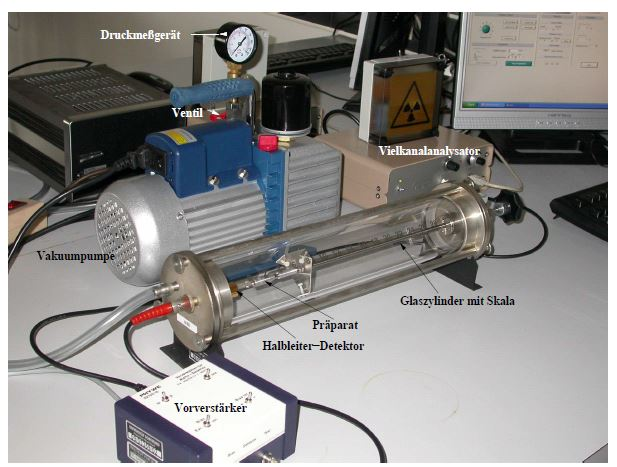
\includegraphics[width = 10cm]{img/Aufbau.JPG}
		\caption{Versuchsaufbau des Experiments \cite{anleitung}.}
		\label{fg:aufbau}
	\end{figure}

	Das Experiment wird nach Abb. \ref{fg:aufbau} aufgebaut.

	In dem evakuierten Glaszylinder befindet sich ein $\alpha$-Strahler, ein Am-Pr"aparat, und ein Detektor.

	Der Abstand zwischen Detektor und Pr"aparat kann "uber einen verschiebbaren Halter an dem Pr"aparat reguliert werden.

	Der Detektor ist ein Halbleiter-Sperrschichtz"ahler, welcher in Abschnitt \ref{sub:halbleiter_sperrschichtz_ahler} beschrieben wurde.

	Der entstehende Impuls wird durch einen Vorverst"arker verst"arkt und einen Vielkanalanalysator entsprechend seiner Pulsh"ohe analysiert.

	Die Daten werden am Computer von dem Programm Multichannel 
	Analyzer verarbeitet.

	Der Schalter bei der Regelung der Me"szeit unten links wird auf AUTO  und unter der Schalter im Programm unter MCA STATUS 
	auf connected gestellt.

	Nun m"ussen die Diskriminatorschwelle am Vielkanalanalysator eingestellt werden. Dazu wird der Abstand Quelle-Detektor auf ein Maximum gestellt und der Abstand so verringert, bis der MCA anf"angt zu z"ahlen.

	\subsection{Durchf"uhrung} % (fold)
	\label{sub:durchf_uhrung}
	

	\subsubsection{Z"ahlrate als Funktion des Drucks} % (fold)
	\label{sub:subsection_name}
	
	Zun"achst wird der Druck in dem Glaszylinder mit Hilfe einer Vakuumpumpe auf etwa $\SI{0}{\milli\bar}$ herabgesenkt.

	Nun wird eine Messung "uber $\SI{120}{\second}$ durchgef"uhrt.

	Bis $\SI{400}{\milli\bar}$ wird der Druck in $\SI{100}{\milli\bar}$-Schritten, von $\SI{400}{\milli\bar}$ bis Normaldruck in $\SI{50}{\milli\bar}$-Schritten variiert und f"ur jeden Druck eine Messung durchgef"uhrt.

	Anschlie"send wird der Abstand um wenige Millimeter vergr"o"sert und die Messung wiederholt.

	\subsection{Statistik des Z"ahlrohrs} % (fold)
	\label{sub:statistik_des_z_ahlrohrs}
	
	Bei etwa $\SI{0}{\milli\bar}$ und dem ersten Abstand aus der vorigen Messung werden 150 Messungen mit einer Me"szeit von etwa $\SI{10}{\second}$ durchgef"uhrt.

	Die gemessenen Werte werden in einem Histogramm mit geschickt gew"ahlter Breite $\Delta N$ aufgetragen und das Ergebnis mit einer Poisson- und einer Gau"sverteilung verglichen.